\documentclass{article}
\usepackage{listings}
\usepackage{graphicx}
\usepackage[slovene]{babel}
\usepackage{color}
\usepackage{amsmath}
\usepackage[usenames,dvipsnames]{xcolor}
\usepackage[hidelinks]{hyperref}
\usepackage{subcaption}
\usepackage{float}
\usepackage{rotating} 
\usepackage{hyperref}
\usepackage{caption}
\usepackage{siunitx}
\graphicspath{{./images/}}

\setlength{\parindent}{0pt}

\begin{document}

\title{Matematično-fizikalni praktikum \\[3mm] \large Naloga 11}
\author{Luka Papež}
\date{18.\ januar 2025}

\begin{center}
    
\includegraphics[width=8cm]{logo-fmf.png}
\end{center}

{
    \let\newpage\relax
    \maketitle
}

\maketitle
\newpage
\section{Naloga}
Izračunaj koeficient $C$.  V ta namen moraš dobiti matriko $A$
in vektor $b$; preuči, kako je natančnost rezultata
(vsote za koeficient $C$) odvisna od števila členov
v indeksih $m$ in $n$. Zaradi ortogonalnosti
po $m$ lahko oba učinka preučuješ neodvisno.

\medskip


Da ima metoda Galerkina določene prednosti celo pred preprostimi
diferenčnimi metodami, opazujmo še na primeru linearne hiperbolične
valovne enačbe v eni dimenziji
\begin{equation*}
  \frac{\partial u}{\partial t} - \frac{\partial u}{\partial \xi} = 0
\end{equation*}
za $\xi \in[0,2\pi]$ s periodičnimi robnimi pogoji.
Začetni pogoj naj bo $u(\xi,0)=\sin(\pi\cos \xi)$;
analitična rešitev enačbe je $u(\xi,t)=\sin(\pi\cos(\xi+t))$.
Primerjaj dobljeni rezultat s tistim, ki ga dobiš,
če prvotno parcialno diferencialno enačbo diskretiziraš
v prvem redu
\begin{equation*}
\frac{u_{i+1,j} - u_{i,j}}{ k} = \frac{u_{i,j+1} - u_{i,j}}{ h}
\end{equation*}
\section{Uvod}
Pri opisu enakomernega laminarnega toka viskozne in nestisljive
tekočine po dolgi ravni cevi pod vplivom stalnega tlačnega
gradienta $p^{\prime}$ se Navier-Stokesova enačba poenostavi
v Poissonovo enačbo
\begin{equation*}
  \nabla^2 v = \Delta v = - \frac{p^\prime}{\eta}\>,
\end{equation*}
kjer je $v$ vzdolžna komponenta hitrosti, odvisna samo  od
koordinat preseka cevi, $\eta$ pa je viskoznost tekočine.
Enačbo rešujemo v notranjosti preseka cevi, medtem ko
je ob stenah hitrost tekočina enaka nič.  Za pretok velja
Poiseuillov zakon
\begin{equation*}
  \Phi = \int_S v\dd S = C\,\frac{p' S^2}{ 8\pi\eta} \>,
\end{equation*}
kjer je koeficient $C$ odvisen samo od oblike preseka cevi
($C=1$ za okroglo cev).  Določili bomo koeficient za
polkrožno cev z radijem $R$. V novih spremenljivkah $\xi=r/R$
in $u=v \eta/(p^\prime R^2)$ se problem glasi
\begin{equation*}
\Delta u(\xi,\phi) = -1 \>,\qquad
u(\xi=1,\phi)=u(\xi,0)=u(\xi,\phi=\pi)=0 \>,
\end{equation*}
\begin{equation*}
  C = 8\pi \iint \frac{u(\xi,\phi)\,\xi\dd \xi \dd\phi}{ (\pi/2)^2} \>.
\end{equation*}

Če poznamo lastne funkcije diferencialnega operatorja za določeno
geometrijo se reševanje parcialnih diferencialnih enačb
včasih lahko prevede na razvoj po lastnih funkcijah. Da bi se izognili
računanju lastnih (za ta primer Besselovih) funkcij in njihovih ničel,
ki jih potrebujemo v razvoju, lahko zapišemo aproksimativno
rešitev kot linearno kombinacijo nekih poskusnih ({\sl trial\/})
funkcij
\begin{equation}
\tilde{u}(\xi,\phi) = \sum\limits_{i=1}^N  a_i \Psi_i(\xi,\phi),
\label{eq:trials}
\end{equation}
za katere ni nujno, da so ortogonalne, pač pa naj zadoščajo
robnim pogojem, tako da jim bo avtomatično zadoščala tudi
vsota (\ref{eq:trials}). Ta pristop nam pride prav v kompleksnejših geometrijah,
ko je uporabnost lastnih funkcij izključena in potrebujemo robustnejši pristop.
Približna funkcija $\tilde{u}$ seveda ne zadosti Poissonovi enačbi: preostane majhna napaka $\varepsilon$
\begin{equation*}
  \Delta \tilde{u}(\xi,\phi) + 1 = \varepsilon(\xi,\phi) \>.
\end{equation*}
Pri metodi Galerkina zahtevamo, da je napaka ortogonalna
na vse poskusne funkcije $\Psi_i$,
\begin{equation*}
  (\varepsilon,\Psi_i) = 0 \>, \qquad  i = 1,2,\dots, N \>.
\end{equation*}
V splošnem bi lahko zahtevali tudi ortogonalnost $\varepsilon$
na nek drug sistem utežnih ({\sl weight\/}) oziroma testnih
({\sl test\/}) funkcij $\Psi_i$.  Metoda Galerkina je poseben
primer takih metod ({\sl Methods of Weighted Residuals\/})
z izbiro $\Psi_i = \Psi_i$.  Omenjena izbira vodi do sistema
enačb za koeficiente $a_i$
\begin{equation}
  \sum_{j=1}^N A_{ij} a_j = b_i\>, \qquad  i = 1,2,\dots, N \>,
  \label{eq:sistem}
\end{equation}
\[
A_{ij} = (\Delta \Psi_j,\Psi_i) \>, \qquad b_i = (-1,\Psi_i) \>,
\]
tako da je koeficient za pretok enak
\begin{equation*}
C =-\frac{32}{ \pi} \sum_{ij}  b_i A_{ij}^{-1} b_j \>.
\end{equation*}
Za kotni del poskusne funkcije obdržimo eksaktne funkcije
$\sin((2m+1)\phi)$, Besselove funkcije za radialni del
pa nadomestimo s preprostejšimi funkcijami $\xi^{2m+1}(1-\xi)^n$.
Pozor: indeks $i$ pomeni seveda dvojni indeks (šteje obenem
$m$ in $n$).  Zaradi ortogonalnosti po $m$ razpade matrika $A$ v bloke,
obrneš pa jo lahko s kako pripravljeno rutino, npr. s spodnjim
in zgornjim trikotnim razcepom {\tt ludcmp} in {\tt lubksb} iz NRC.
\newpage
\section{Rešitev}
\subsection{Računanje geometrijske konstante}
Želimo si izračunati geometrijsko konstanto pretoka skozi polkrožno cev z radijem. To bomo storili z Galerkinovo metodo, ki je opisana v uvodu. Preobrazimo najprej dano vsoto v bolj uporabno obliko.
\begin{equation}
	C =-\frac{32}{ \pi} \sum_{ij}  b_i A_{ij}^{-1} b_j = -\frac{32}{\pi}\vec{b}(A^{-1}\vec{b})=-\frac{32}{pi}\vec{b}\vec{a}
\end{equation}
Nato si pomagamo z analitičnimi rešitvami in konstruiramo ortogonalne poskusne funkcije $\Psi_{mn}(\xi,\phi) = \xi^{2m+1}(1-\xi)^n \sin((2m+1)\phi)$. Z nekaj računanja tako definiramo matriko $A$ in $\vec{b}$ in z reševanjem sistema $A\vec{a}=\vec{b}$ dobimo $\vec{a}$ in nato še enostavno vrednost konstante $C$.
\begin{align}
	A_{(m'n')(mn)} &= (\Delta\Psi_{mn}, \Psi_{m'n'}) = -\frac{\pi}{2}\delta_{m'm}\frac{nn'(3+4m)}{2+4m+n+n'}B(n+n'-1,3+4m) \\
	b_{(m'n')} &= (-1, \Psi_{m'n'}) = -\frac{2}{2m'+1}B(2m'+3,n'+1)
\end{align}
Da dobimo nekaj občutka za problem si najprej poglejmo kakšno obliko ima nekaj poskusnih funkcij.
\begin{figure}[H]
    \centering
    \begin{subfigure}[b]{0.49\textwidth}
        \centering
        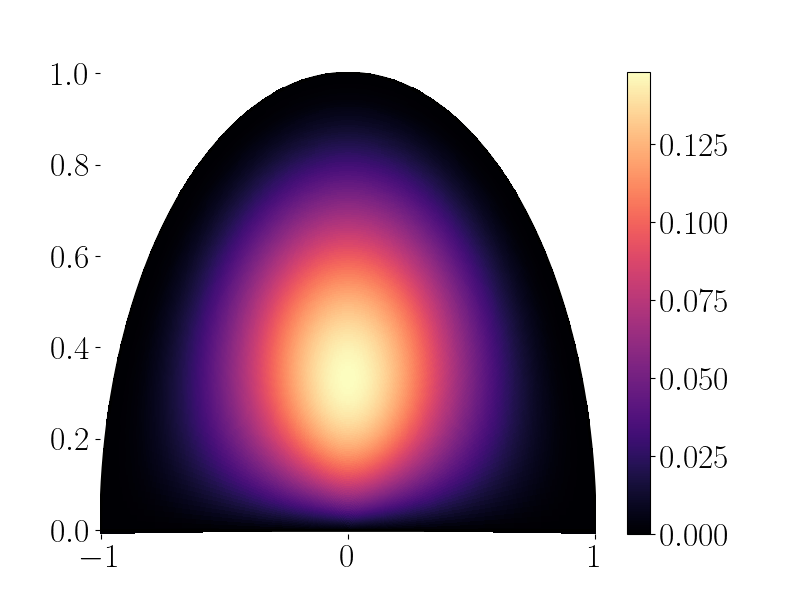
\includegraphics[width=\linewidth]{pretok0-2.png}
		\caption{Poskusna funkcija $m=0$ in $n=2$}
    \end{subfigure}
    \hfill
    \begin{subfigure}[b]{0.49\textwidth}
        \centering
        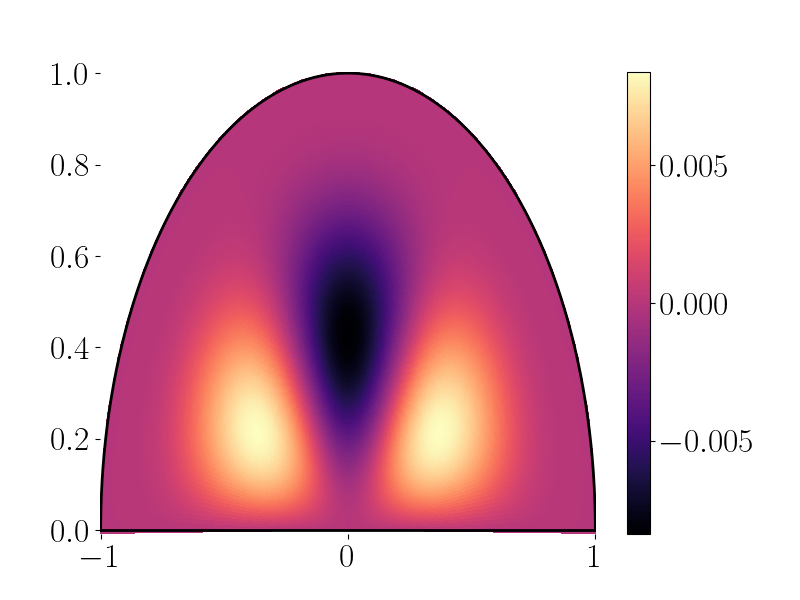
\includegraphics[width=\linewidth]{pretok1-4.png}
        \caption{Poskusna funkcija $m=1$ in $n=4$}
    \end{subfigure}
    \caption{Vizualizacija poskusnih funkcij sistema}
\end{figure}
Iz podanih vizualizacij lahko naredimo nekaj predpostavk o njihovem obnašanju. Opazimo namreč, da z večanjem konstant dobimo več `skupin` toka in da se red velikosti pri višjih konstantah precej zmanjša. Rešimo zdaj sistem $A\vec{a}=\vec{b}$ in si poglejmo kakšna je naša numerična rešitev.
\begin{figure}[H]
	\centering
	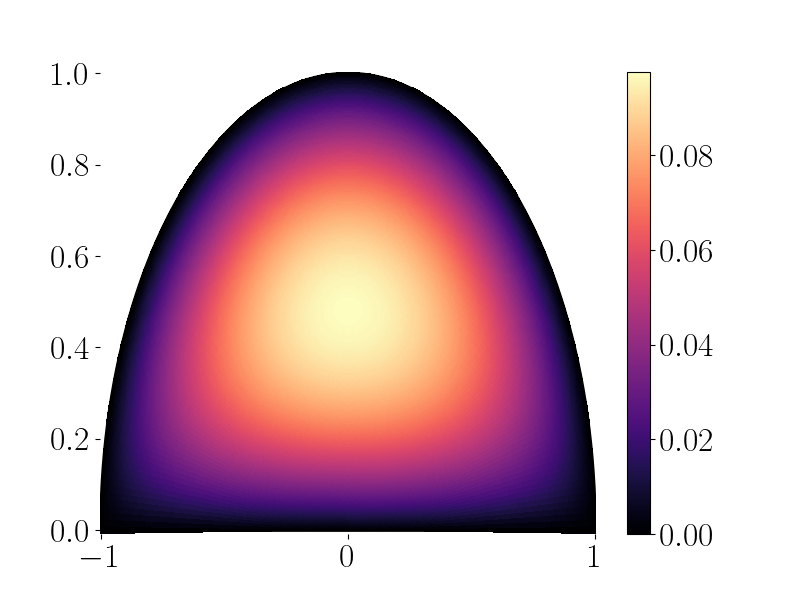
\includegraphics[width=0.6\linewidth]{pretok.png}
	\caption{Numerična rešitev hitrostnega polja}
\end{figure}
Dobimo lepo rešitev, kjer je na sredini hitrost največja in se postopoma zmanjšuje proti robovom. Zanimivi del naše polkrožne geometrije pa je krožni rob okoli $\phi=0$ in $\phi=\pi$, kjer nastane večje počasnejše območje. V primerjavi s poskusnimi funkcijami pred vsem opazimo, da v njihovi linearni kombinaciji ni več negativnih območji, kar nam pravi tudi intuicija. Poleg tega je območje večjih hitrosti tudi precej večje in se bolj približa robu. 

\smallskip

Iz rešenega matričnega sistema enačb zdaj zlahkoto izračunamo še vrednost geometrijske konstante $C$. Seveda se moremo najprej vprašati koliko členov neskončne vsote potrebujemo za željeno natančnost. Zaradi ortogonalnosti po $m$ lahko obe konstanti $m$ in $n$, ki določata število členov, opazujemo neodvisno, kar precej olajša časovno zahtevnost. Po kratkem igranju z vrednostmi ugotovimo, da nas omejitve spomina omejijo na približno $n=150, m=150$. Da ocenimo napako vzamemo vrednost z največ členi in pogledamo kako tiste z manj členi konvergirajo k njej.
\newpage
\begin{figure}[H]
    \centering
    \begin{subfigure}[b]{0.49\textwidth}
        \centering
        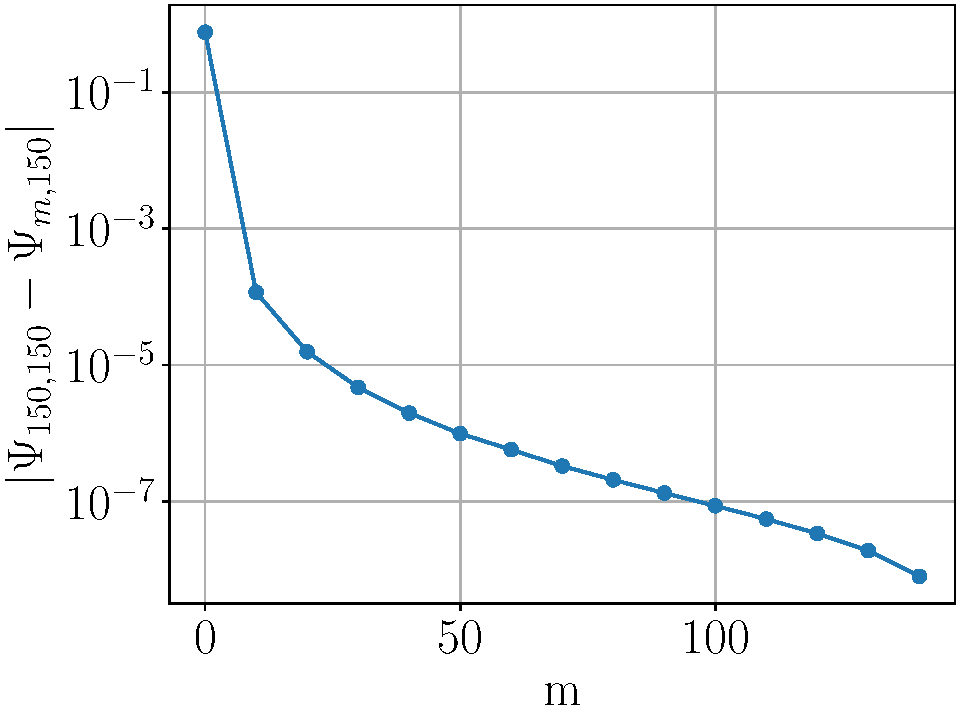
\includegraphics[width=\linewidth]{mprecision.pdf}
		\caption{Odstopanje s parametrom $m$ in $n=150$}
    \end{subfigure}
    \hfill
    \begin{subfigure}[b]{0.49\textwidth}
        \centering
        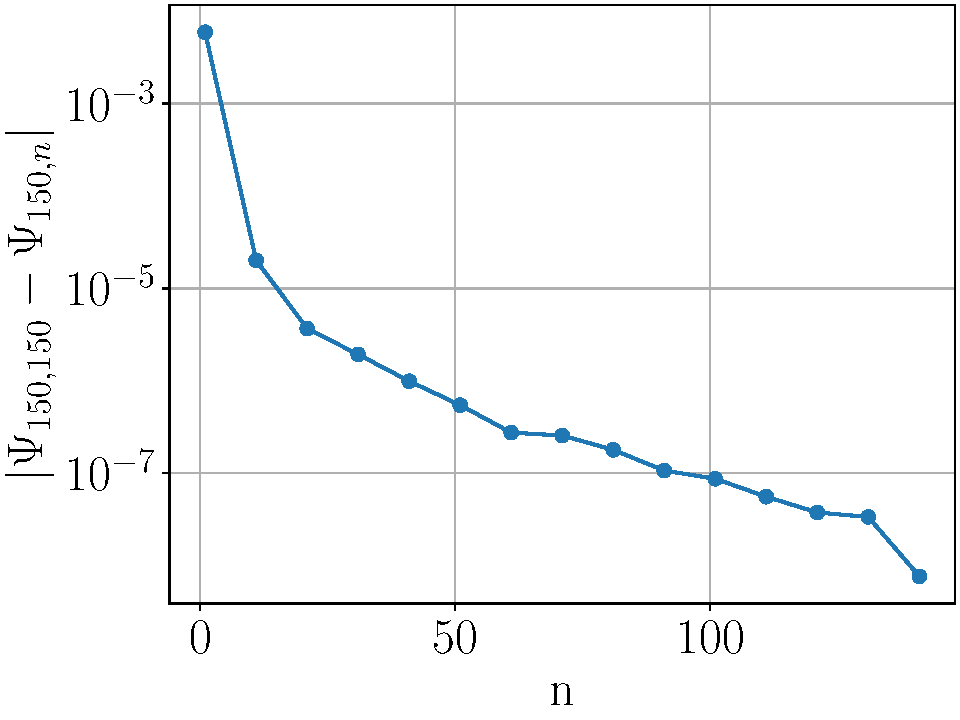
\includegraphics[width=\linewidth]{nprecision.pdf}
		\caption{Odstopanje s parametrom $n$ in $m=150$}
    \end{subfigure}
	\caption{Odstopanje od vrednosti $C$ z $n=150$ in $m=150$}
\end{figure}
Z dobljenimi grafi opazimo, da odvisnost odstopanja v obeh primerih pade pod $10^{-7}$ pri vrednosti parametra $100$. Pri višjih vrednostih pa se večanje natančnosti upočasni in tako pri $n=150$ in $m=150$ z gotovostjo napovemo $6$ do $7$ decimalk in sicer $C=0.7577220$.
\subsection{Reševanje linearne hiperbolične valovne enačbe}
Rešimo še linearno hiperbolično valovno enačbo v eni dimenziji \\$\frac{\partial u}{\partial t} - \frac{\partial u}{\partial \xi} = 0$. Želimo namreč pokazati, da ima metoda Galerkina nekatere prednosti pred diferenčnimi metodami. Omejimo se na območje $\xi \in [0, 2\pi]$ z začetnimi pogoji $u(\xi, 0) = \sin{(\pi \cos{\xi})}$. Analitična rešitev enačbe je namreč $u(\xi, t)=\sin{(\pi \cos{(\xi + t)})}$. Tako razvijemo po poskusnih funkcijah $\Psi_j(\xi)$ v vsoto, ki formira $u(\xi, t)$ in zahtevamo po Galerkinu 
\begin{equation}
	\int_0^{2\pi} \left[ \frac{\partial u}{\partial t} - \frac{\partial u}{\partial \xi} \right] \Psi_k^*(\xi) \, \mathrm{d}\xi = 0.
\end{equation}
Za poskusne funkcije izberemo ravne valove $\Psi_j(\xi)=\frac{1}{\sqrt{2\pi}}e^{ij\xi}$. Funkcijo $u$ pa nato dobimo preko Galerkinove zahteve, iz katere sledi sistem enačb za koeficiente razvoja $a_j$ po funkcijah $\Psi_j(\xi)$. 
\begin{equation}
	\frac{da_k}{dt}=ika_k, k=-N/2,...,N/2
\end{equation}
Tako za izračun potrebujemo le še začetni pogoj za koeficiente $a_k(0)=\int_0^{2\pi}u(\xi, 0)\Psi^*(\xi)d\xi$, kar lahko rešimo s trapezno metodo. Diferencialno enačbo pa rešimo s pomočjo metode Runge-Kutta-45. To pa bomo primerjali še z diferenčnim prostopom $\frac{u_{i+1,j}-u_{i, j}}{k} = \frac{u_{i, j+1} - u_{i, j}}{h}$.
\newpage
Začnimo seveda z analitično rešitvijo, kjer nam razvoj po ravnih funkcijah, da koeficiente $a_k(t) = \sin{(\frac{k\pi}{2})J_k(\pi)e^{ikt}}$.
\begin{figure}[H]
    \centering
    \begin{subfigure}[b]{0.49\textwidth}
        \centering
        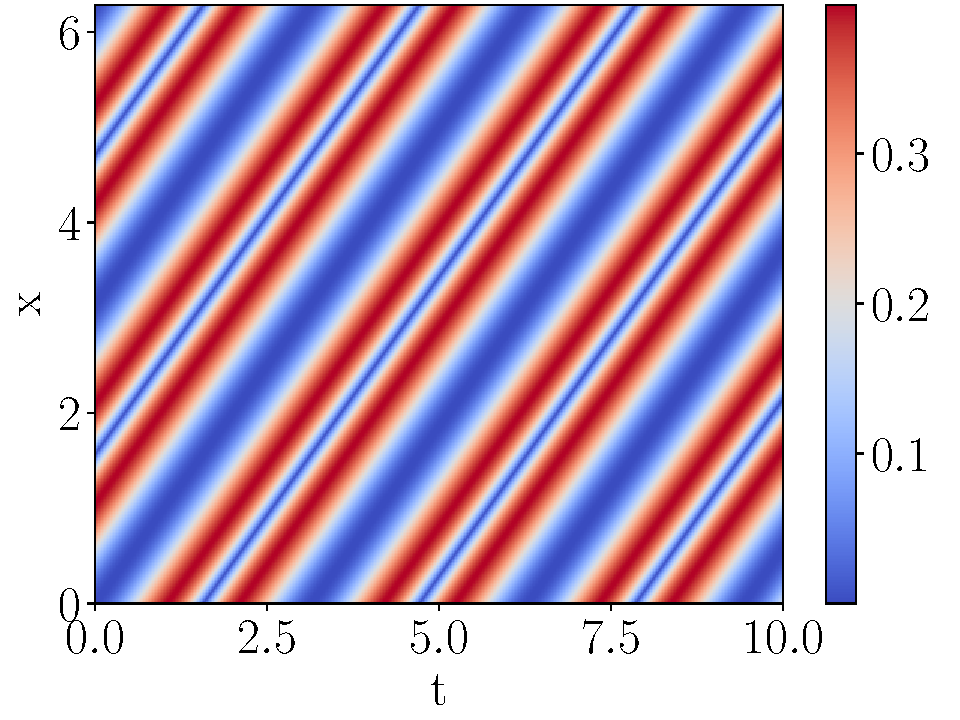
\includegraphics[width=\linewidth]{waveanal2d.pdf}
		\caption{2D vizualizacija}
    \end{subfigure}
    \hfill
    \begin{subfigure}[b]{0.49\textwidth}
        \centering
        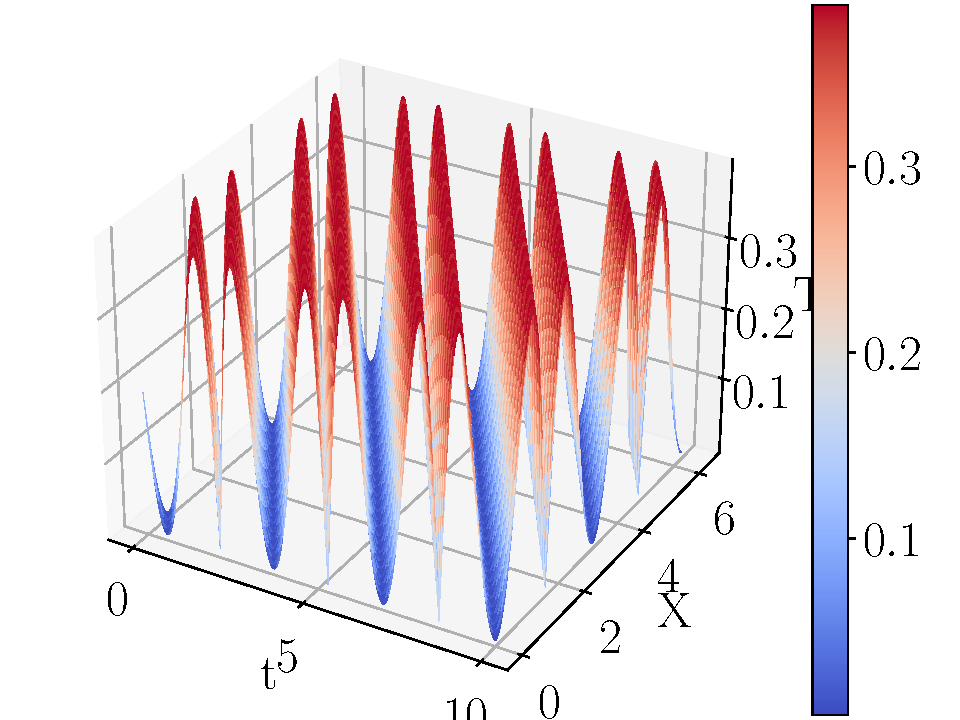
\includegraphics[width=\linewidth]{waveanal3d.pdf}
		\caption{3D vizualizacija}
    \end{subfigure}
	\caption{Absolutna vrednost analitične rešitve linearne hiperbolične parcialne diferencialne enačbe.}
\end{figure}
Opazimo že poznano obliko, kjer se valovi postopoma pomikajo naprej. Poglejmo kako numerične rešitve odstopajo od numeričnih.
\begin{figure}[H]
    \centering
    \begin{subfigure}[b]{0.49\textwidth}
        \centering
        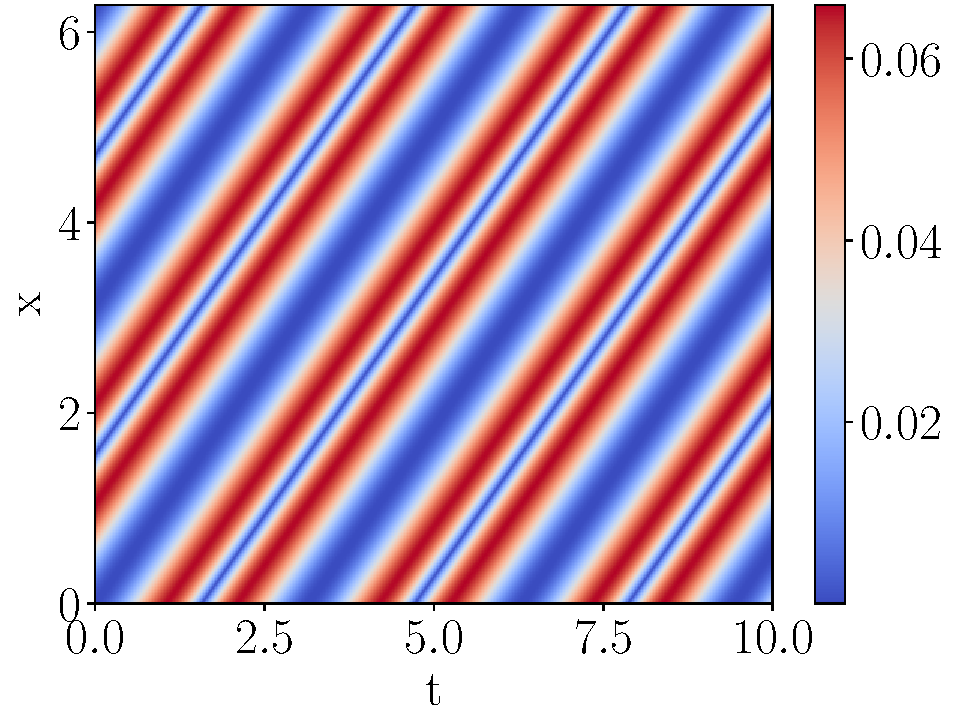
\includegraphics[width=\linewidth]{wavegalerkin2d.pdf}
		\caption{Galerkinova metoda}
    \end{subfigure}
    \hfill
    \begin{subfigure}[b]{0.49\textwidth}
        \centering
        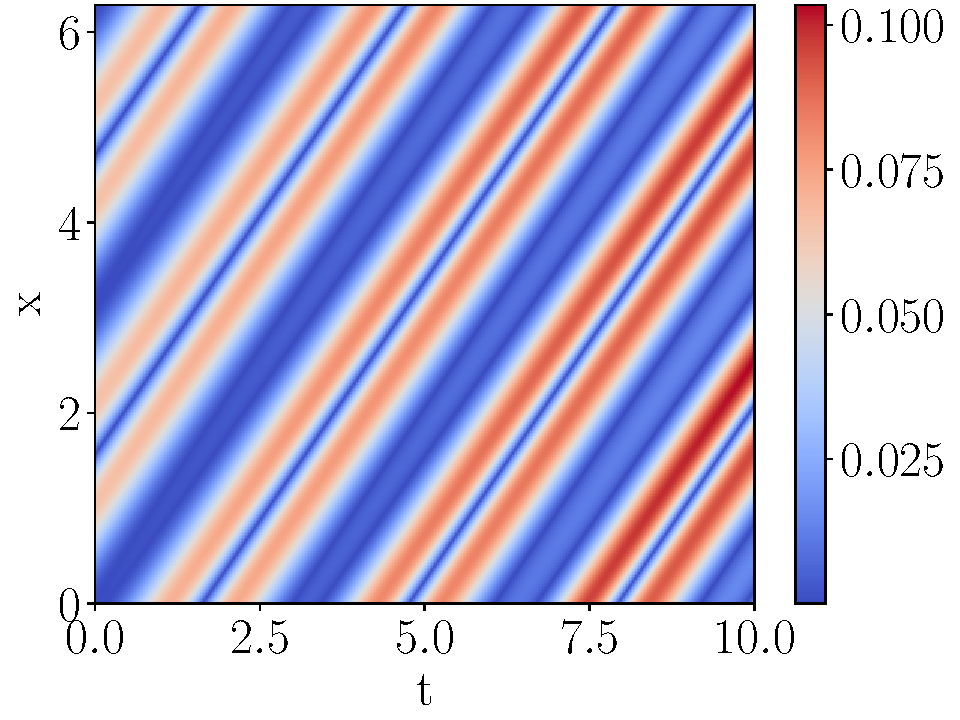
\includegraphics[width=\linewidth]{wavediff2d.pdf}
		\caption{Diferencialna metoda}
    \end{subfigure}
	\caption{Absolutna vredost odstopanja numeričnih rešitev linearne hiperbolične parcialne diferencialne enačbe od analitične rešitve}
\end{figure}
Tako pridemo do zaključka, da obe metodi kar precej dobro simulirata premikanje valovanja. Odstopanje od analitične rešitve in medseboj se namreč skriva predvsem v amplitudi valov, kjer se Galerkinova metoda izkaže za bolj stabilno v primerjavi z diferencialno.
\section{Zaključek}
Tako smo zaključil še z zadnjo nalogo v skupini numeričnega reševanja parcialnih diferencialnih enačb. Reševanje njih mi je postalo kar precej zanimivo. Nekoliko je k temu pripomoglo tudi predavanje o protieksplozijski zaščiti pri Industrijski fiziki, kjer so nam bili pokazane simulacije eksplozij z metodami, ki smo jih obravnavali. \href{https://brr.fyi/posts/south-pole-signage}{Zaključujem še s povezavo do znakov, ki jih najdemo na južnem polu.}
\end{document}
